\documentclass[11pt]{report}
\title{MATH-36032 PSBC Project 3: Purchasing Data Analysis}

\setlength\parindent{0pt}

\usepackage[utf8]{inputenc}
\usepackage{amsmath}
\usepackage{amssymb}
\usepackage{amsthm}
\usepackage{listings}
\usepackage[margin=0.8in]{geometry}
\usepackage{xcolor}
\usepackage{graphicx}
\usepackage{enumerate}
\usepackage{esvect}

\usepackage{titlesec}
\titleformat{\chapter}[hang]
{\normalfont\LARGE\bfseries}{\chaptertitlename\ \thechapter.}{1em}{}

\definecolor{codegreen}{rgb}{0,0.6,0}
\definecolor{codegray}{rgb}{0.5,0.5,0.5}
\definecolor{codepurple}{rgb}{0.58,0,0.82}
\definecolor{backcolour}{rgb}{0.95,0.95,0.92}
 
\lstdefinestyle{mystyle}{
    backgroundcolor=\color{backcolour},
    commentstyle=\color{codegreen},
    keywordstyle=\color{blue},
    numberstyle=\tiny\color{codegray},
    stringstyle=\color{codepurple},
    basicstyle=\ttfamily\footnotesize,
    breakatwhitespace=false,
    breaklines=true,
    captionpos=b,
    keepspaces=true,
    numbers=left,
    numbersep=5pt,
    showspaces=false,
    showstringspaces=false,
    showtabs=false,
    tabsize=2,
    columns=fullflexible,
    numberbychapter=false
}
\usepackage{titlesec}
\renewcommand{\chaptername}{}

\titlespacing{\chapter}{-8pt}{0pt}{15pt}

\newcommand{\block}[1]{
  \underbrace{1 \cdots 1}_{#1}
}
\lstset{style=mystyle}

\makeatletter
\renewcommand*\env@matrix[1][\arraystretch]{%
  \edef\arraystretch{#1}%
  \hskip -\arraycolsep
  \let\@ifnextchar\new@ifnextchar
  \array{*\c@MaxMatrixCols c}}
\makeatother

\begin{document}

\section*{MATH-36032 PSBC Project 3: Purchasing Data Analysis}
This project seeks to analyse a dataset collected over a four-year period, for some of the active customers of a large online retailer. The data is provided in a comma separated values (CSV) format. The following information is available in the dataset. 

\begin{itemize}
	\item \texttt{Date:} Online transaction date from 1\textsuperscript{st} January 2015 to 31\textsuperscript{st} December 2018.
	\item \texttt{Customer\_ID:} Anonymised customer ID.
	\item \texttt{Product\_Category:} Category of the product from 5 categories tagged \texttt{A-E}.
	\item \texttt{Product\_Value:} The total amount of the order in British pounds (£).
	\item \texttt{Rating:} Customer rating from \texttt{1-5}. Any sales for which a rating was not provided have the value \texttt{0}.
	\item \texttt{Return:} \texttt{Y} (Yes) or \texttt{N} (No) indicating if the product was returned for a refund.
\end{itemize}


The first few entries in the dataset can be seen below.

\begin{table}[ht!]
\begin{center}
\begin{tabular}{cccccc}
\texttt{Date,} & \texttt{Customer\_ID,} & \texttt{Product\_Category,} & \texttt{Product\_Value,} & \texttt{Rating,} & \texttt{Return;} \\
\texttt{01-Jan-2015,} & \texttt{1010408,} & \texttt{B,} & \texttt{33.5,} & \texttt{5,} & \texttt{N;} \\
\texttt{01-Jan-2015,} & \texttt{1014220,} & \texttt{C,} & \texttt{18.4,} & \texttt{4,} & \texttt{N;} \\
\texttt{01-Jan-2015,} & \texttt{1016167,} & \texttt{E,} & \texttt{23.2,} & \texttt{4,} & \texttt{N;} \\
\texttt{01-Jan-2015,} & \texttt{1019094,} & \texttt{D,} & \texttt{46,} & \texttt{0,} & \texttt{Y;}
\end{tabular}
\end{center}
\end{table}

This project tackles the following three problems. \\

% ******************************** TASK 1 ******************************** %
{\let\clearpage\relax \chapter{Logistic Regression}}
%\chapter{Logistic Regression}
% ------ Problem ------ %
\section*{Problem}
Majority of the customers who returned the product gave a low rating. Let $P(r)$ be the probability that a product is likely to be returned. We seek to find a relationship between $P(r)$ and the rating $r$, given by the customer in the following \emph{logistic function} with two parameters $\alpha$ and $\beta$.

\begin{equation}
	P(r) = \frac{1}{1 + \exp(-\alpha r - \beta)}.
\end{equation}

% ------ Approach ------ %
\section{Approach}
The two parameters $\alpha$ and $\beta$ can be obtained by minimising a loss function. A loss function is a measure of how well a prediction model performs in predicting the expected outcome, i.e. a smaller value of the loss function implies a better performance. From the several loss functions available, we minimise the `Sum of Squares' loss function which is defined as follows:

\begin{equation}
	\sum_{i}{(P_i - P(r_i))^2}.
	\label{eq:loss_func}
\end{equation}

Suppose we have a MATLAB function \texttt{sumsquareloss}, which implements the loss function defined in (\ref{eq:loss_func}). \\

\lstinputlisting[language=Matlab, caption={Implementation of Sum of Squares loss function defined in (\ref{eq:loss_func}).},label={lst:sumsquareloss}]{sumsquareloss.m}

We can use the \texttt{fminsearch} function in MATLAB to minimise \texttt{sumsquareloss} as a function of $\alpha$ and $\beta$. However, it is necessary to perform some pre-processing on the given dataset before we can optimise the logistic regression function.

\subsection{Pre-processing}
In order to reduce the overall computational complexity, we only consider ratings given by those customers who have returned an order at least once. To extract this data from the dataset, we first gather the \texttt{Customer\_ID}'s of all the orders that were returned. Using this result, we can obtain all the orders belonging to those customers only. Once we have this sub-table, we can remove any orders that were not rated by the customer, i.e. $\texttt{Rating}=0$. \\

Finally, we can extract the array \texttt{ratings}, and the corresponding array \texttt{probs}, containing logical values 1 or 0 which represents whether the product was returned or not. These can be used as the input parameters \texttt{r} and \texttt{p} for the \texttt{sumsquareloss(a,r,p)} function.

\subsection{Implementation}
Upon the pre-processing of the data, we make use of the \texttt{fminsearch} and \texttt{sumsquareloss} functions to minimise the loss in the logistic regression model and find the parameters $\alpha$ and $\beta$. The proposed function, \texttt{LogisticFunction()} serves the purpose. \\

\lstinputlisting[language=Matlab, caption={\texttt{LogisticFunction()} returns the parameters $\alpha$ and $\beta$ in $P(r)$.}, label={lst:logfunc}]{LogisticFunction.m}


% ------ Results ------ %
\section{Result}
The \texttt{LogisticFunction()} returns the two parameters $\alpha$ and $\beta$. In particular, the optimised parameters for the model are calculated as the following. \\

\begin{lstlisting}[title={Output of \texttt{LogisticFunction()}.}]
>> LogisticFunction()

ans = -17.542411276527133  17.418797309784775
\end{lstlisting}
 
The output from the function yields the values $\alpha=-17.5424$ (4dp) and $\beta=17.4188$ (4dp). Figure \ref{fig:logreg} depicts a plot of the logistic regression function calculated above. It is evident that a low rating of 1 has a high probability, $P(r)$, which was what was expected. 

\begin{figure}[h]
	\centering
	\noindent\makebox[\textwidth]{
  	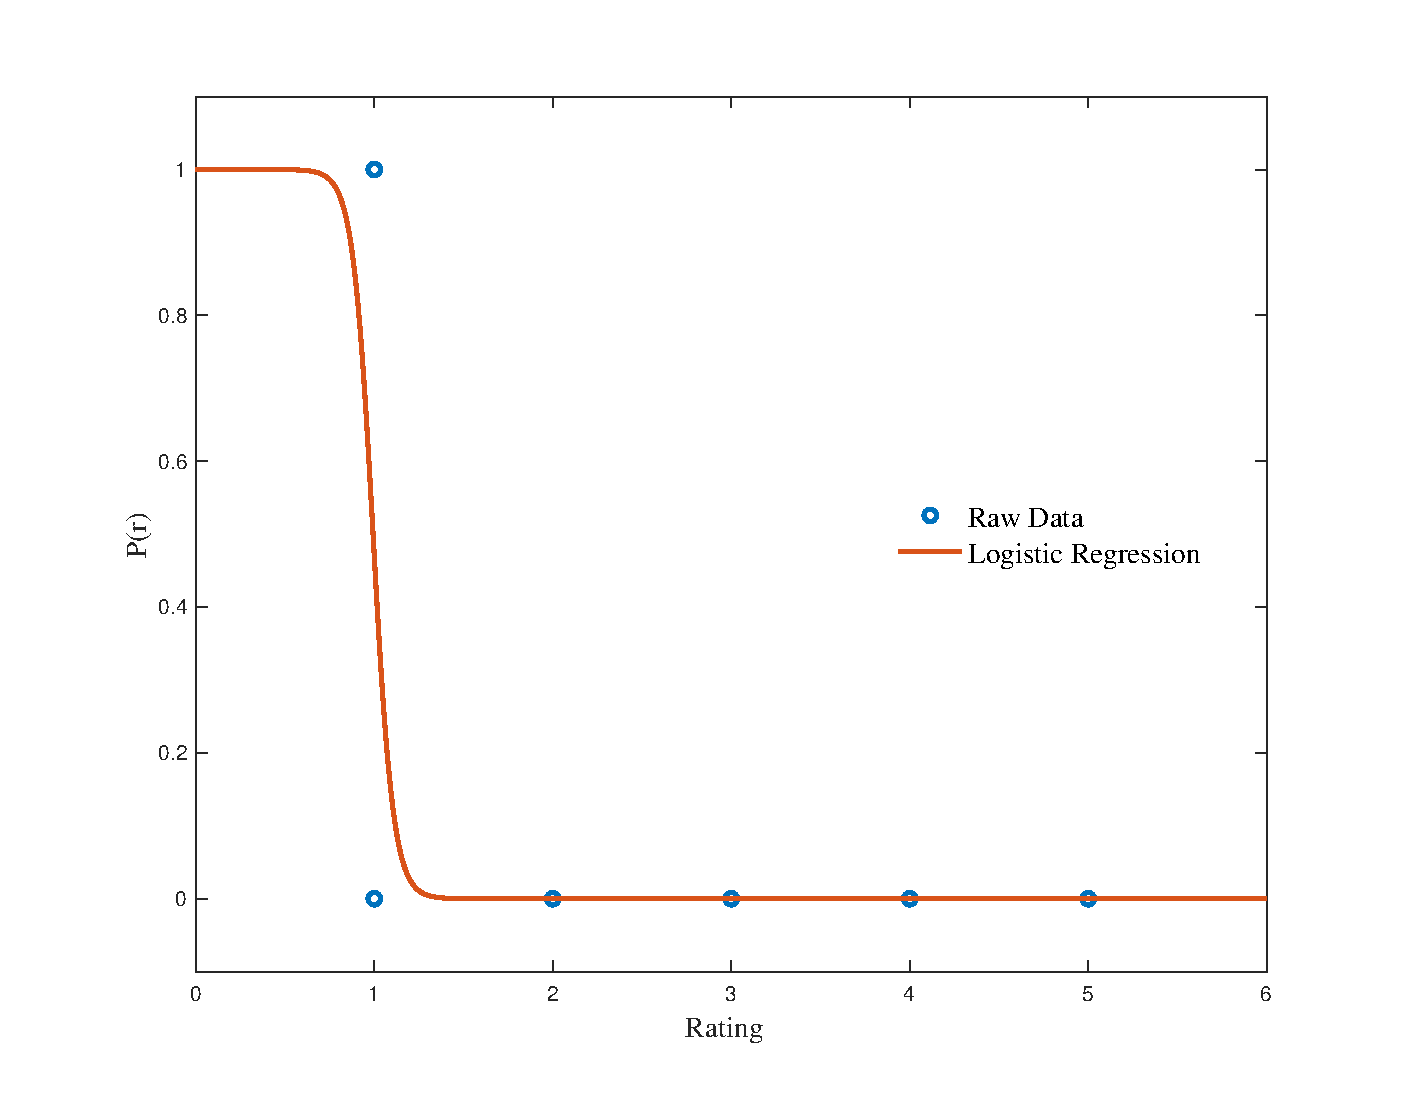
\includegraphics[scale=0.75]{assets/logreg}}
  	\caption{Plot of the Logistic Regression function.}
  	\label{fig:logreg}
\end{figure}

% ******************************** TASK 2 ******************************** %
\chapter{Returning Customers}
% ------ Problem ------ %
\section*{Problem}
It is intuitive to believe that if a customer returns a product, they are less likely to make future orders from the company. The aim of this task is to investigate if this is actually the case by defining a suitable likelihood criteria.

% ------ Approach ------ %
\section{Approach}
First of all, we define the criteria for the likelihood that a customer will make another purchase after returning a product. We define this such that the likelihood of a customer making future orders is measured by the percentage of total amount spent after the return, over the total amount spent over the four year period, excluding the refunded orders.

\subsection{Implementation}
Suppose we have the following function \texttt{ReturningLikelihood()} which returns an overall likelihood that customers who made one return, placed another order in the future. This is showcased below. \\

\lstinputlisting[language=Matlab, caption={\texttt{ReturningLikelihood()} returns an overall likelihood (\%) of customers returning after a refunded order.},label={lst:return_likelihood}]{ReturningLikelihood.m}

\subsection{Correctedness}
\begin{proof}[\unskip\nopunct]
	The function first extracts all the transactions that were returned (line 7). From this, all the unique \texttt{Customer\_ID}'s of such customers are obtained in an array (line 8). The function then loops over this list of \texttt{Customer\_ID}'s. In each iteration, i.e. for each customer, all orders placed by that customer are retrieved (line 12). This is further refined to orders that were not returned and the total amount spent by the customer (\texttt{total\_spent}) is calculated (line 13-14). The date of the first order returned by the customer is obtained and the total amount spent after that date (\texttt{spent\_after\_return}), excluding refunded orders, is calculated (line 15-17). Finally, the \texttt{likelihood} array that corresponds to the customer ID's is populated with the ratio, $\texttt{spent\_after\_return}/ \texttt{total\_spent}$ (line 18).\\
	
	Once the likelihood for each customer is calculated, it is converted to a percentage (line 20) and then a mean of these likelihoods is returned by the function (line 21). Hence, we successfully calculate the desired likelihood.
\end{proof}

% ------ Results ------ %
\section{Result}
The output of the \texttt{ReturningLikelihood()} function is an overall percentage representing the likelihood of a customer making another purchase after they have returned an order.

\begin{lstlisting}[title={Output of \texttt{ReturningLikelihood()}.}]
>> ReturningLikelihood()
ans = 50.421477089777326
\end{lstlisting}

The average likelihood is approximately $50\%$, which is not the best indication whether the customer is less likely to come back after returning an order. Therefore, we plot a histogram to analyse the distribution of likelihoods for all such customers. Figure \ref{fig:histogram} depicts the histogram.

\begin{figure}[h]
	\centering
	\noindent\makebox[\textwidth]{
  	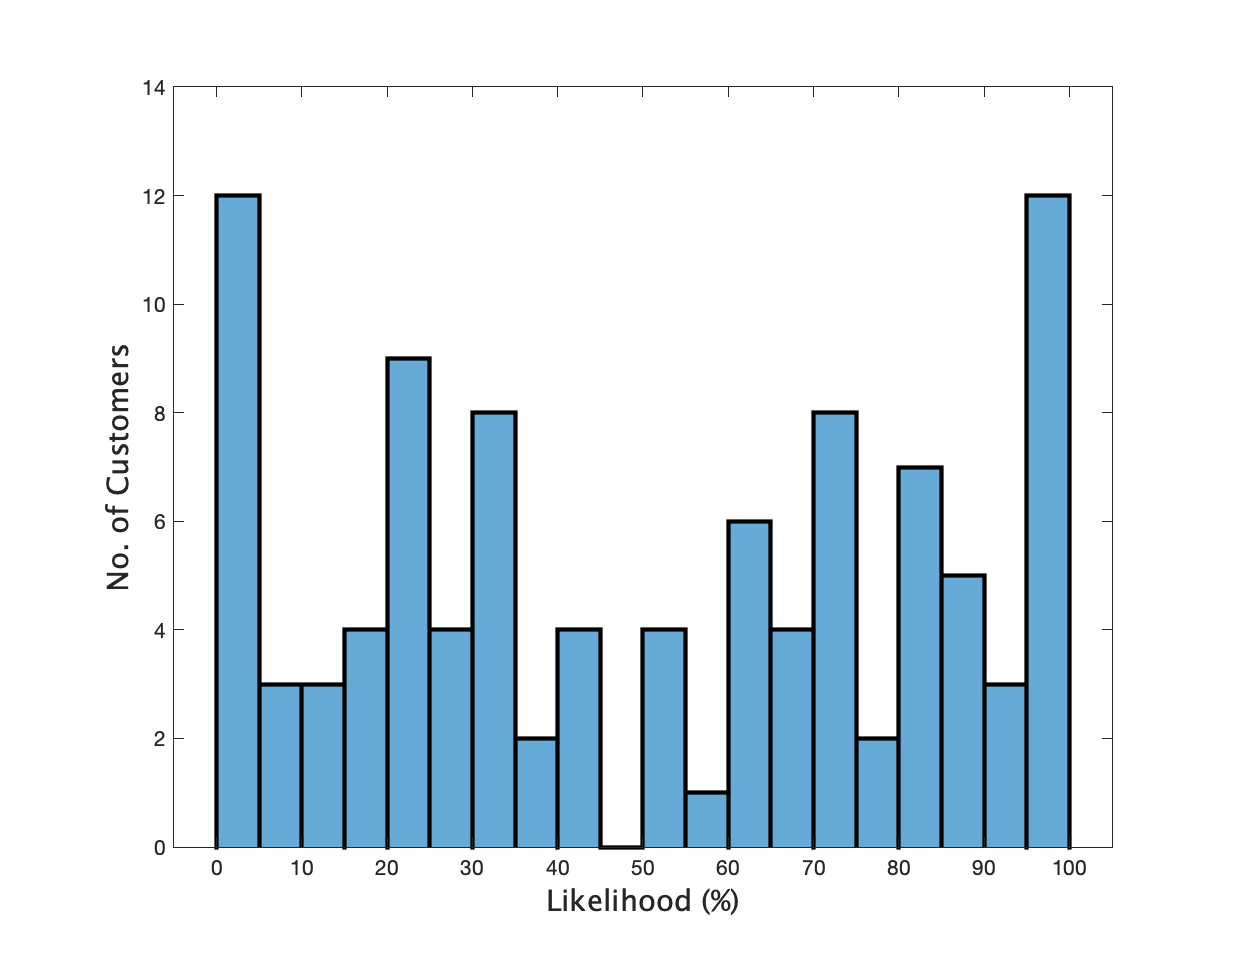
\includegraphics[scale=0.5]{assets/histogram}}
  	\caption{Distribution of likelihoods.}
  	\label{fig:histogram}
\end{figure}

We consider the original intuition that customers are less likely to make another purchase after a refunded order. If this was the case, the histogram would be a triangular shape with the peak closer to a likelihood of 0\% ($x=0$). However, this is not the case as illustrated by Figure \ref{fig:histogram}. Hence, we can conclude that the customers are not necessarily less likely to make a purchase after having a product returned.

\paragraph{\textbf{NB:}} It is important to note that the \texttt{ReturningLikelihood()} function is implemented to only consider the date of the first order that is returned. However, a customer could have multiple returns. Therefore, it will be a better indicator to consider the average of the amounts spent in all the segments between these return dates. This was not implemented in this function because in the given dataset, none of the customers made more than one refund.

% ******************************** TASK 3 ******************************** %
\chapter{Loyalty Reward}
% ------ Problem ------ %
\section*{Problem}
The company has decided to send 100 coupons with $30\%$ off for clothing in product category C, to build a long-term customer loyalty and to manage inventory more effectively. The customers who have placed orders with large values in category C, and have given higher ratings are the targets for these coupons. The aim of the task is to rank the customers based on a weighted average of following two criteria:

\begin{enumerate}[ {(}I{)} ]
	\item Average amount spent per order in Category \texttt{'C'}.
	\item The average rating given for such orders.
\end{enumerate}

The weights must be chosen in such a way such that the customers ranked at the top according to either (I) or (II) independently are still likely to be at the top with both (I) and (II) combined.

% ------ Approach ------ %
\section{Approach}
Since the rankings are based on two separate variables, we must find a way to normalise these into a weighting where they can be used together. The approach we take is to normalise the average amount spent and the ratings given, so that they are both values between 0 and 1. Once we have values between 0 and 1 for the rating and the amount spent for each customer, we can add the two normalised values together and rank the customers according to the highest sum. The customers with the highest sum will be ranked at the top. This approach allows us to compare both the \texttt{Rating} and the \texttt{Product\_Value} equally because they are both values between 0 and 1. Hence, adding those together would give a reasonable indicator of rank. \\

The average \texttt{Product\_Value} for each customer is normalised by dividing by the most expensive order value. On the other hand, \texttt{Rating} is divided by 5 (highest possible rating).

\subsection{Implementation}
Suppose we have a function \texttt{RankCustomers()}, which returns the ranked list of customers that have placed orders in product category C. To implement such a function, we first obtain all the orders placed in category C. We can use this to retrieve all the unique \texttt{Customer\_ID}'s and make use of the \texttt{accumarray} function in MATLAB to get a mean of the total value spent and the mean ratings given for each customer. These averages can then be normalised as discussed above and generate a table with \texttt{Customer\_ID}'s and their corresponding normalised average product value (\texttt{norm\_value}), average rating (\texttt{norm\_rating}) and the sum (\texttt{norm\_sum}). The function is implemented as follows. \\

\lstinputlisting[language=Matlab, caption={\texttt{RankCustomer()} returns the customers ranked in order.},label={lst:rank_customers}]{RankCustomers.m}

% ------ Results ------ %
\section{Result}
The \texttt{RankCustomers()} function outputs a table in order of rankings for all the customers who made a purchase in product category C. The top 10 and the customers ranked from 91-100 are outputted below as a result of \texttt{RankCustomers()}. \\

\begin{lstlisting}[title={Rankings of customers calculated by \texttt{RankCustomers()}.}, language=MATLAB]
>> rankings = RankCustomers();

% Top 10 Customers
>> rankings(1:10,:)
ans =
    customer_id       norm_value        norm_rating        norm_sum    
    ___________    _________________    ___________    ________________
      1014288      0.998784933171324          1        1.99878493317132
      1011981      0.992709599027947          1        1.99270959902795
      1016309      0.875455650060753          1        1.87545565006075
      1014429      0.838396111786148          1        1.83839611178615
      1012195      0.814702308626975          1        1.81470230862697
      1016443      0.806804374240583          1        1.80680437424058
      1015864      0.800121506682868          1        1.80012150668287
      1014953                      1        0.8                     1.8
      1014887      0.792223572296476          1        1.79222357229648
      1011918      0.772782503037667          1        1.77278250303767

% Rank 91-100 Customers
>> rankings(91:100,:)
ans =
    customer_id       norm_value        norm_rating        norm_sum    
    ___________    _________________    ___________    ________________
      1010573      0.572296476306197        0.9         1.4722964763062
      1015326      0.621506682867558       0.85        1.47150668286756
      1013142      0.471445929526124          1        1.47144592952612
      1012489      0.468408262454435          1        1.46840826245444
      1013800      0.515188335358445       0.95        1.46518833535844
      1011041       0.46415552855407          1        1.46415552855407
      1011068      0.462940461725395          1        1.46294046172539
      1017300       0.86269744835966        0.6        1.46269744835966
      1011436      0.461725394896719          1        1.46172539489672
      1013998      0.461117861482382          1        1.46111786148238
\end{lstlisting}


We can see in the top 10 result above that both the \texttt{norm\_value} and \texttt{norm\_rating} values are very close to 1. One of the requirements of the rankings was that the rankings must be similar to the cases where criteria (I) and (II) are considered independently. To validate this, we plot the normalised average product value against the rating, highlighting the points that were picked as the top 100 customers. A good weighting of both criteria would result in selecting the points towards the top right-hand triangular region of the graph, as this region indicates that the rankings will be similar if considered independently. Figure \ref{fig:rankings} depicts the result of all such customers. It is clear to see that the top 100 chosen customers are in the top-right region, indicating that the rankings are somewhat optimal.

\begin{figure}[h]
	\centering
	\noindent\makebox[\textwidth]{
  	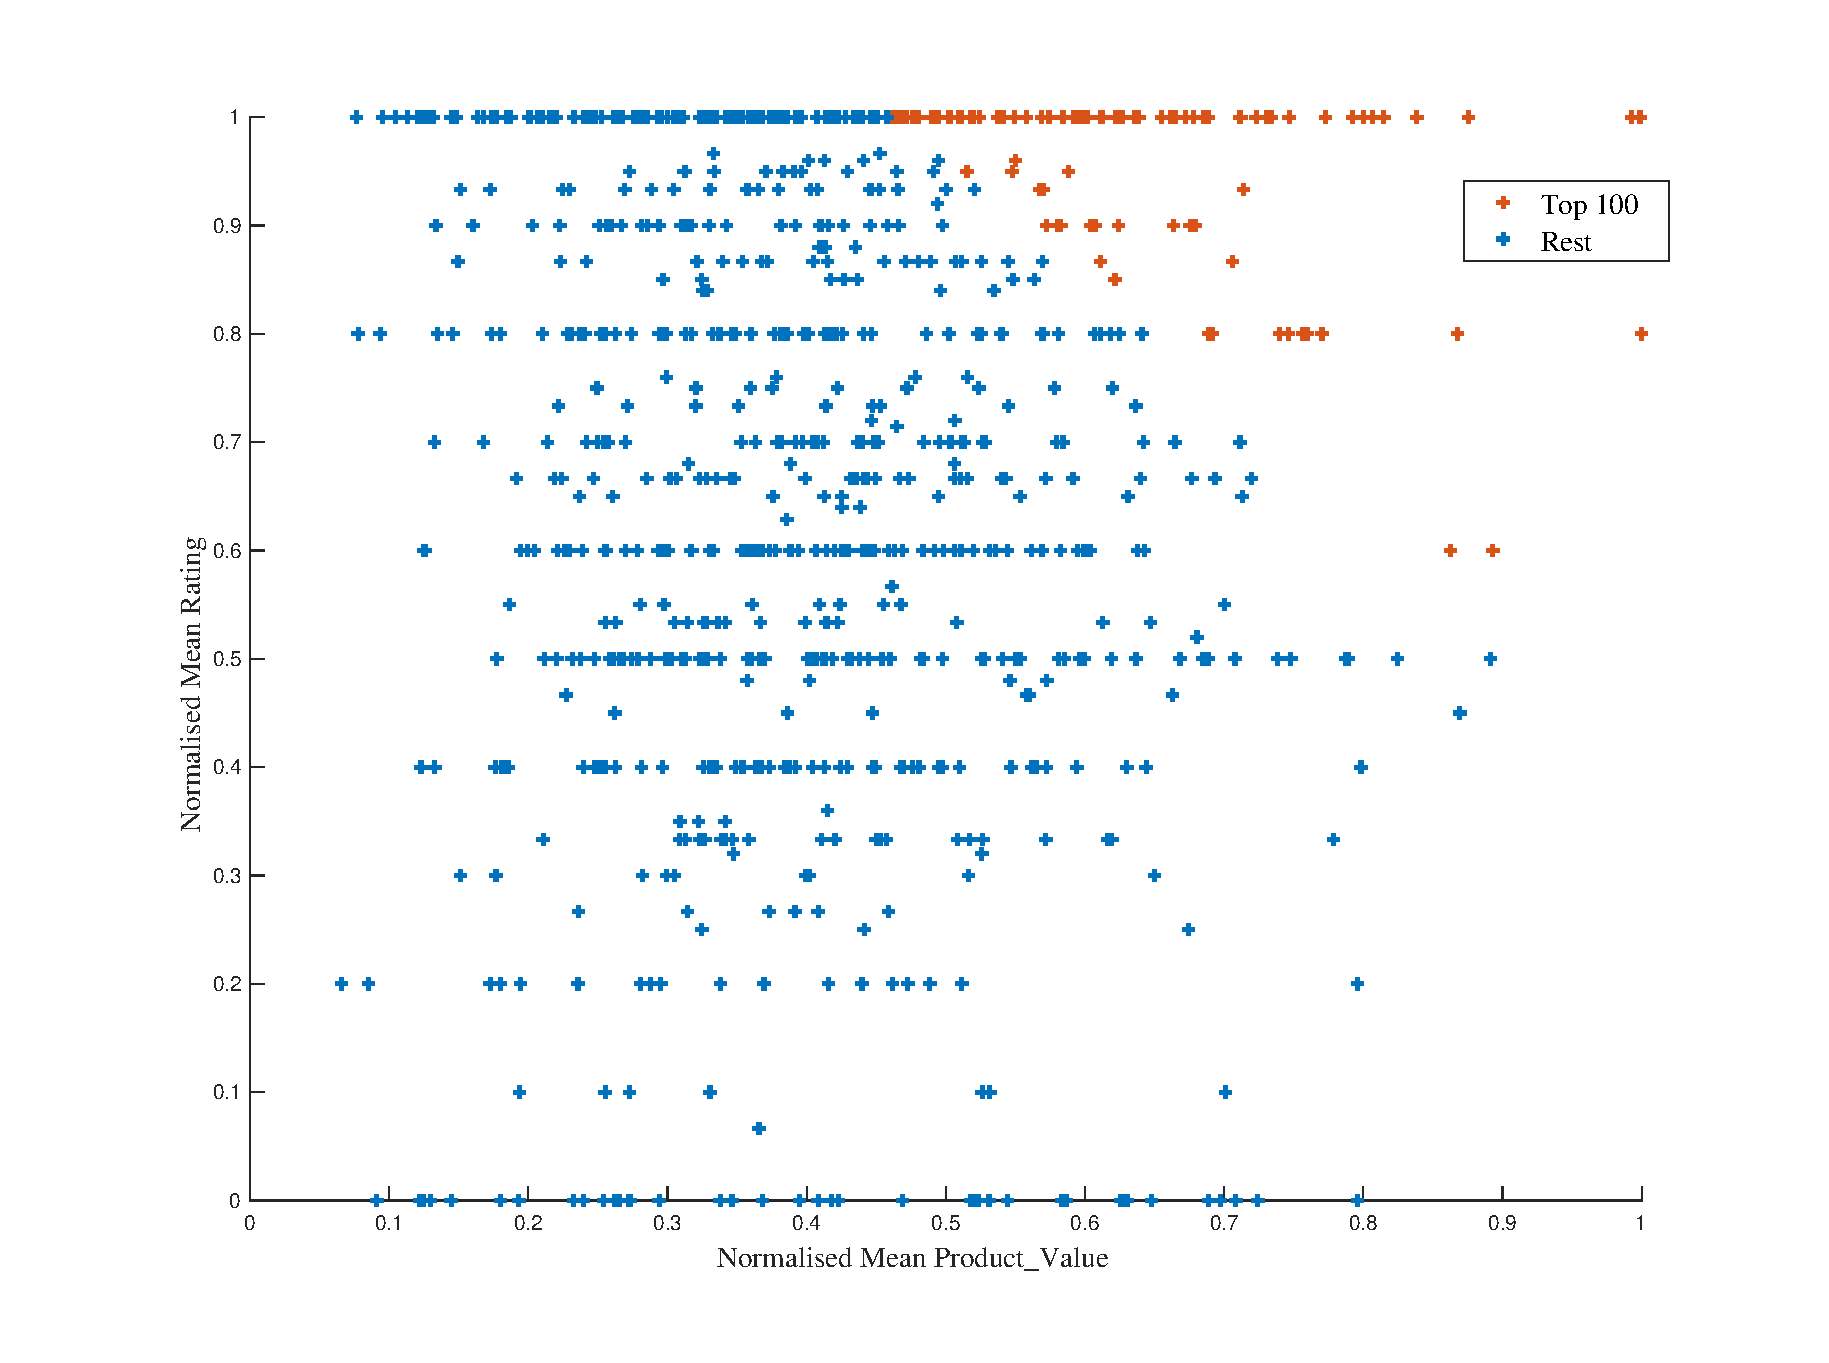
\includegraphics[scale=0.7]{assets/rankings}}
  	\caption{Normalised Product Value (\texttt{norm\_value}) vs. Rating (\texttt{norm\_rating}), highlighting the top 100 customers.}
  	\label{fig:rankings}
\end{figure}

\end{document}
